\documentclass{beamer}
\usetheme{Lab2C}
\usepackage{graphicx}
\usepackage{subcaption}
\usepackage{amsfonts}
\usepackage{amsmath}
\usepackage{amsthm}
\usepackage{algorithm}
\usepackage{algorithmic}
\usepackage{bm}
\usepackage{hyperref}
\usepackage{footmisc}
\usepackage{xcolor}
\DeclareMathOperator\E{\mathbb{E}}
\DeclareMathOperator\Var{\mathrm{Var}}
\def\R{\mathbb{R}}
\def\P{\mathcal{P}}
\usepackage{mathtools}
\DeclarePairedDelimiter\abs{\lvert}{\rvert}
\DeclarePairedDelimiter\norm{\lVert}{\rVert}
\DeclarePairedDelimiter\inner{\langle}{\rangle}
\def\red#1{\textcolor{red}{#1}}
\makeatletter
\newcommand{\algorithmicfunction}{\textbf{function}}
\newcommand{\algorithmicendfunction}{\algorithmicend\ \algorithmicfunction}
\newenvironment{ALC@func}{\begin{ALC@g}}{\end{ALC@g}}
\newcommand{\FUNCTION}[2][default]{\ALC@it\algorithmicfunction\ #2\ %
\textbf{:}%
\ALC@com{#1}\begin{ALC@func}}
\ifthenelse{\boolean{ALC@noend}}{
    \newcommand{\ENDFUNCTION}{\end{ALC@func}}
  }{
    \newcommand{\ENDFUNCTION}{\end{ALC@func}\ALC@it\algorithmicendfunction}
  }
\makeatother
\theoremstyle{definition}
\newtheorem{definition}{Definition}
\newtheorem{theorem}{Theorem}
\newtheorem{example}{Example}
\newtheorem{corollary}{Corollary}
\newtheorem{lemma}{Lemma}
\newtheorem{remark}{Remark}
%further improvement
%background intro added Chen Chuan's work
%simulation add hierarchical method
%find suitable dataset to apply info-clustering
%Yang Li's suggestion: compared with other clustering method, the threshold is the same or not
%early stopping technique, complexity from n -> log(n)
\title{A Graph-Based Information Theoretic Clustering Method}
\author{Feng Zhao\inst{1} \and Yang Li\inst{2} \and Shao-Lun Huang\inst{2}}
\institute{\inst{1}Dept. of Electronic Engineering, Tsinghua University
\and \inst{2}Tsinghua-Berkeley Shenzhen Institute, Tsinghua University}
\date{\today}
\begin{document}
\begin{frame}
	\titlepage
\end{frame}
\section*{Outline}
\begin{frame}
	\tableofcontents
\end{frame}

\section{Introduction}
\subsection{Overview of existing clustering method}
\begin{frame}
\frametitle{Existing clustering method}
\begin{figure}
    \centering
    \begin{subfigure}[b]{0.3\textwidth}
        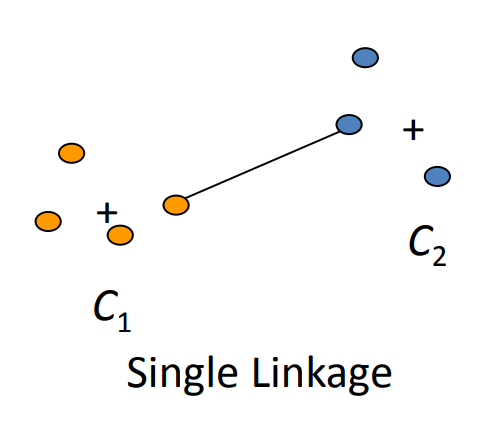
\includegraphics[width=\textwidth]{pic/agglomerative.png}
        \caption{Agglomerative method}
    \end{subfigure}~
    \begin{subfigure}[b]{0.3\textwidth}
        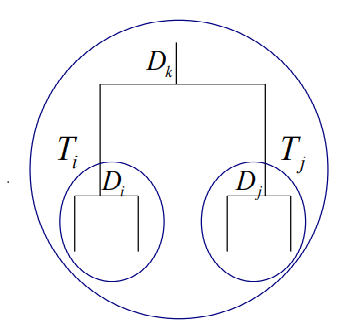
\includegraphics[width=\textwidth]{pic/bayesian.png}
        \caption{Bayesian method}
    \end{subfigure}
    ~ %add desired spacing between images, e. g. ~, \quad, \qquad, \hfill etc. 
    %(or a blank line to force the subfigure onto a new line)
    \begin{subfigure}[b]{0.3\textwidth}
        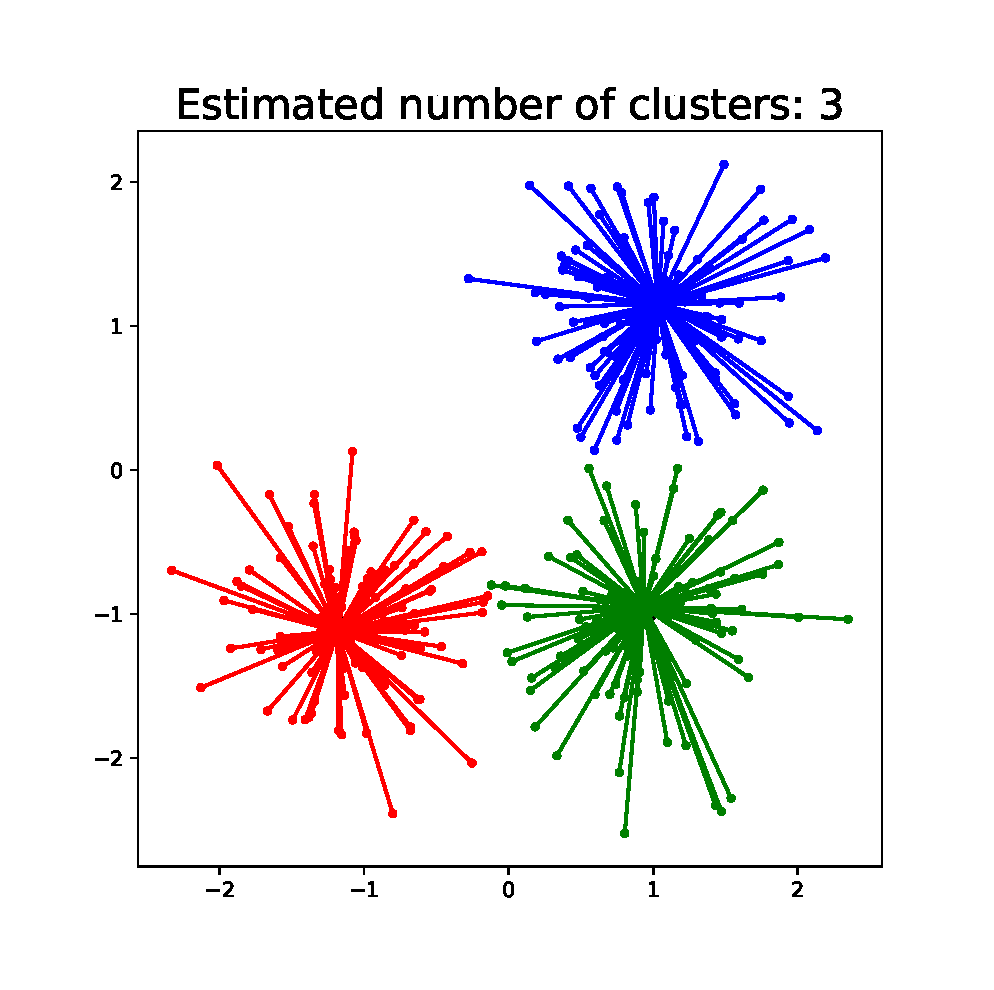
\includegraphics[width=\textwidth]{pic/affinity_propagation.eps}
        \caption{Affinity propagation}
    \end{subfigure}
\end{figure}
\end{frame}

\begin{frame}
\frametitle{Problems}
\begin{itemize}
\item binary hierarchical tree only.
\item probabilistic model
\begin{itemize}
\item many hyper-parameters to tune 
\item need many reruns
\end{itemize}
\item many graph-based methods are not hierarchical.
\end{itemize}
\end{frame}

\subsection{Mutual Similarity and its extension}
\begin{frame}
\begin{block}{mutual similarity}
\begin{itemize}
\item Gaussian kernel $ \exp({-\gamma \norm{p_1 - p_2}^2})$
\item threshold distance $\delta(\norm{p_1-p_2} < \delta^*)$
\end{itemize}
\end{block}

\begin{definition}[Multivariate Similarity]
Given a graph $G(V, E)$, with vertex as data point, edge weight as mutual similarity, the multivariate similarity $I(Z_V)$
\begin{align}
I(Z_V) & = \min_{\mathcal{P} \in \Pi'(V)} I_{\mathcal{P}}(Z_V) \\
\label{eq:newDef}  I_{\mathcal{P}}(Z_V) & = \frac{1}{ \abs{\mathcal{P}} - 1} \sum_{\substack{i\in C, j \not\in C\\ C\in \mathcal{P}, (i,j) \in E}} w_{ij}
\end{align}
\end{definition}
\end{frame}
\begin{frame}
\frametitle{Illustrative example}
\begin{columns}
\column{5cm}
\begin{figure}
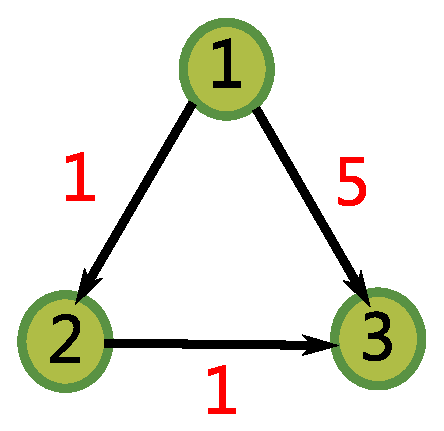
\includegraphics[width=4cm]{pic/example_directed.eps}
\end{figure}
\column{5cm}
\begin{align*}
I_{\{1\},\{2\},\{3\}}(Z_{\{1,2,3\}}) & = 3.5 \\
I_{\{1,3\},\{2\}}(Z_{\{1,2,3\}}) & = 2 \\ 
I_{\{1,2\},\{3\}}(Z_{\{1,2,3\}}) & = 6 \\ 
I_{\{1\},\{2,3\}}(Z_{\{1,2,3\}}) & = 6 \\ 
\Rightarrow I(Z_{\{1,2,3\}}) & = 2 \\
\end{align*}
\begin{equation*}
I(Z_{\{1,3\}}) = 5, I(Z_{\{1,2\}}) = 1
\end{equation*}
\end{columns}
\end{frame}
%\section{B matrix and its relationship with multivariate mutual information}

\begin{frame}{Hierachical clustering method}

\begin{description}
\item[top-down] $I_{\P^*}(Z_V)=I(Z_V)$ and use $\P^*$ to split.
\item[bottom-up] $I(Z_C) = \max_{B\subseteq V} I(Z_B)$ and use $C$ to merge.
\end{description}
\begin{figure}
\centering
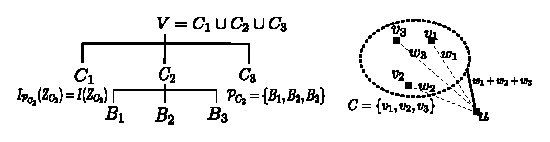
\includegraphics[width=\textwidth]{paper/pic/two_approach.eps}
\caption{Left: top-down approach. Right: bottom-up approach}
\end{figure}
\end{frame}
\begin{frame}
\frametitle{Illustrative example}
\begin{figure}
\centering
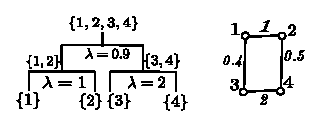
\includegraphics[width=0.7\textwidth]{paper/pic/threshold.eps}
\caption{a clustering tree (left) for the weighted graph (right)}
\end{figure}

The threshold values $\lambda$ are $I(Z_{3,4})=2, I(Z_{1,2})=1$ and $I(Z_V)=0.9$ respectively.
\begin{equation*}
\P = 
\begin{cases}
\{\{1,2,3,4\}\} & \lambda < 0.9 \\
\{\{1,2\},\{3,4\}\} & 0.9 \leq \lambda < 1 \\
\{\{1\},\{2\},\{3,4\}\} & 1 \leq \lambda < 2\\
\{\{1\},\{2\},\{3\},\{4\}\} & \lambda \geq 2
\end{cases}
\end{equation*}
\end{frame}
\section{Algorithms}
\begin{frame}
\begin{definition}[graph cut function]
$C$ is a subset of $V$:
\begin{align}
f(C) & = \sum_{i\not\in C, j \in C, (i,j) \in E} w_{ij} \\
f[\P] & = \sum_{C \in \P} f(C)
\end{align}
\end{definition}
\begin{theorem}
\begin{equation}\label{eq:hLambda}
h(\lambda) = \min_{\P \in \Pi(V)} \{ f[\P] - \abs{\P}\lambda \}
\end{equation}
The optimal partitions $\P_1, \dots, \P_k$ for $h(\lambda)$ are nested such that $\P_1 \succeq \P_2 \dots \succeq \P_k$, and we can obtain the hierarchical clustering tree from this sequence.
\end{theorem}
\end{frame}
\begin{frame}
\frametitle{Illustrative Example}
\begin{columns}
\column{5cm}
\begin{figure}
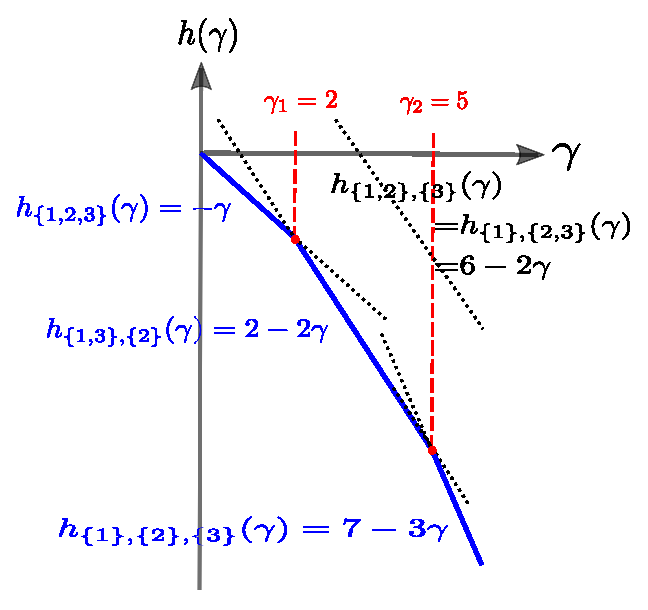
\includegraphics[width=5cm]{pic/dt.eps}
\caption{piecewise linear function $h(\gamma)$}
\end{figure}
\column{5cm}
\begin{align*}
h(\lambda)  & = \min_{\P} h_{\lambda}(\P) \\
h_{\lambda}(\P) & = f[\P] - \abs{\P}\lambda
\end{align*}
\begin{align*}
\P_0  & = \{\{1,2,3\}\} \\
\P_1  & = \{\{1,3\},\{2\}\} \\
\P_2  & = \{\{1\},\{2\},\{3\}\} 
\end{align*}

\end{columns}
\end{frame}
\begin{frame}
\begin{columns}
\column{4cm}
\begin{figure}[!ht]
\centering
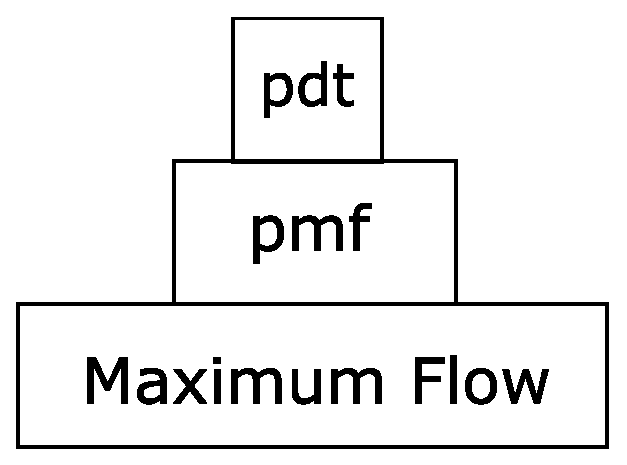
\includegraphics[width=4cm]{paper/pic/pdt.eps}
\caption{pyramid structure of graph-based info-clustering algorithm}\label{fig:ps}
\end{figure}
\column{6cm}
\begin{enumerate}
\item parametric Dilworth truncation: $\min \{f[\P] -\lambda \abs{\P}\}$
\item parametric maximum flow: $\min_{t\in C} \{f(C) - \lambda - y^{\lambda}(C)\}$
\item maximum flow
\end{enumerate}
Achievable time complexity: $\abs{V}^3 \sqrt{\abs{E}}$
% For push-relabel algorithm, \mathrm{MF}(G(V,E)) = \abs{V}^2 E
\end{columns}
\end{frame}
\begin{frame}
	\frametitle{Solving $\min_{t\in C} \{f(C) - \lambda - y^{\lambda}(C)\}$}
	\begin{columns}
		\column{5cm}
		\column{5cm}
	\end{columns}
	
\end{frame}
\section{Numerical Results}
\begin{frame}
\begin{figure}[!ht]
\centering
\begin{subfigure}{\textwidth}
\IfFileExists{code/utility/build/4part.eps}
{\includegraphics[width=12cm]{code/utility/build/4part.eps}}
{\includegraphics[width=12cm]{pic/4part.eps}} % not up-to-date

\caption{Illustrative example from four Gaussians}\label{fig:4p}
\end{subfigure}
\begin{subfigure}{\textwidth}
\IfFileExists{code/utility/build/3circle.eps}
{\includegraphics[width=12cm]{code/utility/build/3circle.eps}}
{\includegraphics[width=12cm]{pic/3circle.eps}} % not up-to-date
\caption{Illustrative example from three circles}\label{fig:3c}
\end{subfigure}
\end{figure}
\end{frame}
\begin{frame}
\frametitle{empirical comparision}
\begin{table}[!ht]
\centering
\InputIfFileExists{build/compare.tex}{}{}
\caption{clustering accuracy for info-clustering and existing algorithms}
\end{table}
\end{frame}
\section{Conclusion and Contribution}
\begin{frame}
\frametitle{Conclusion}
\begin{itemize}
\item propose multivariate information, used in info-clustering method
\item implement info-clustering algorithm
\item competitive with existing algorithms in some dataset
\end{itemize}
\end{frame}
\section{Reference}
\begin{frame}
\frametitle{Further Reading}
\begin{thebibliography}{9}
\bibitem{ic} Chung Chan, \newblock Info-Clustering: A Mathematical Theory for Data Clustering
\newblock  IEEE Transactions on Molecular, Biological and Multi-Scale Communications, June 2016
\bibitem{pin}  Chung Chan, \newblock Info-Clustering: An Efficient Algorithm by Network Information Flow
\newblock 2017 Information Theory and Applications Workshop (ITA)
\bibitem{mac} Kiyohito Nagano \newblock Minimum Average Cost Clustering \newblock NIPS 2010
\end{thebibliography}
\end{frame}
\end{document}
